% !TeX root = ../paper.tex
\hypertarget{experiments}{%
\section{Experiments}\label{experiments}}

Unless otherwise specified, SmartVLA results are reported using the corresponding
target-domain-adapted experts. For LIBERO, LIBERO-Plus, LIBERO-Pro, and RoboTwin2.0, we follow the
evaluation settings released with each benchmark. LIBERO-SMART task contracts and scoring are
specified in Appendix~\ref{appendix:smart-benchmark}; the Piper real-robot protocol is described in
Appendix~\ref{appendix:real-robot-piper}. The overall evaluation scope is summarized in
Figure~\ref{fig:overview}(d). All success rates are reported as percentages.

\subsection{LIBERO-SMART}\label{libero-smart-1}

% !TeX root = ../paper.tex
\begin{table}[htbp]
\centering
\setlength{\abovecaptionskip}{0pt}
\setlength{\belowcaptionskip}{\baselineskip}
\caption{LIBERO-SMART success rates (\%). $\dagger$ denotes an agentic system.}
\label{tab:libero-smart}
\label{tab:agentic-smart}
\nointerlineskip
\normalsize
\setlength{\tabcolsep}{3.6pt}
\begin{tabular}{@{}lrrrrr@{}}
\toprule
Method & Sem & Vis & Con & Avg. & Goal-only \\
\midrule
OpenVLA-OFT & 1.45 & 0.30 & 1.15 & 0.97 & 1.65 \\
$\pi_{0}$ & 0.00 & 0.00 & 0.00 & 0.00 & 0.85 \\
$\pi_{0.5}$ & 14.70 & 2.00 & 4.85 & 7.18 & 17.92 \\
X-VLA & 0.00 & 0.00 & 0.00 & 0.00 & 0.55 \\
GR00T N1.6 & 8.35 & 0.80 & 1.00 & 3.38 & 13.22 \\
StarVLA & 12.60 & 1.95 & 4.00 & 6.18 & 15.62 \\
CaP-X$^\dagger$ & 12.75 & 6.75 & \textbf{21.25} & 13.58 & 18.33 \\
Agentic+$\pi_{0.5}^{\dagger}$ & 17.75 & 3.50 & 14.25 & 11.83 & 18.22 \\
\midrule
\rowcolor{smartvlarow}
\textbf{SmartVLA-Pi} & 23.05 & \textbf{8.40} & 12.55 & 14.67 & 29.73 \\
\rowcolor{smartvlarow}
\textbf{SmartVLA-OFT} & 20.10 & 5.55 & 16.45 & 14.03 & 32.73 \\
\rowcolor{smartvlarow}
\textbf{Agentic+SmartVLA-Pi$^\dagger$} & \textbf{26.50} & 7.00 & 19.50 & \textbf{17.67} & \textbf{37.97} \\
\bottomrule
\end{tabular}
\end{table}
%

\Needspace{14\baselineskip}
% !TeX root = ../paper.tex
\begin{wrapfigure}[14]{r}{0.51\textwidth}
\centering
\setlength{\parskip}{0pt}
\setlength{\abovecaptionskip}{\baselineskip}
\setlength{\belowcaptionskip}{0pt}
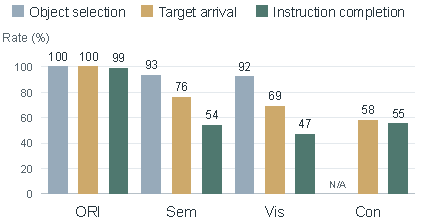
\includegraphics[width=\linewidth]{figures/fig3_behavior_diagnosis.pdf}\par\nointerlineskip
\caption{SmartVLA-Pi behavioral diagnosis (\%).}
\label{fig:smartvla-behavior}
\end{wrapfigure}
%

% Start the wrapped paragraph without overriding the style's line-breaking settings.
\begingroup
\leavevmode
Table~\ref{tab:libero-smart} evaluates whether SmartVLA improves the three instruction-following
capabilities targeted by our method. In direct-policy evaluation, SmartVLA-Pi and SmartVLA-OFT
achieve average success rates of 14.67\% and 14.03\%, compared with 7.18\% for $\pi_{0.5}$, with
improvements across all three suites. The Semantic gains indicate better execution of local commands
and instruction-specific constraints; the Visual Prompt gains reflect improved use of visually
specified objects and target locations; and the Control gains show better adjustment to commands
issued during execution. These improvements are consistent with learning segment-aligned commands
and visual prompts as conditions for subsequent actions. Under Goal-only scoring, which checks
any-time goal attainment without the additional contract requirements, the two variants also improve
from 17.92\% for $\pi_{0.5}$ to 29.73\% and 32.73\%. Their advantage therefore extends beyond the
strict scoring criterion.
\par
\endgroup

\paragraph{Behavioral diagnosis.}

Figure~\ref{fig:smartvla-behavior} revisits the motivating interventions with SmartVLA-Pi.
Instruction-completion rates increase from 6.00\%, 5.00\%, and 25.00\% for $\pi_{0.5}$ to 54.00\%,
47.00\%, and 55.00\% on Semantic, Visual Prompt, and Control, respectively, while original-task
completion remains at 99.00\%. This comparison connects the benchmark improvements to more reliable
execution of local instructions, visual prompts, and command updates.

Under a fixed agentic protocol, replacing $\pi_{0.5}$ with SmartVLA-Pi raises strict system success
from 11.83\% to 17.67\% and Goal-only success from 18.22\% to 37.97\%. Thus, improved low-level
instruction following also benefits systems that invoke the policy through an upper-level
controller. Calling and scoring protocols are detailed in Appendices~\ref{agentic-calling-protocol}
and~\ref{app:smart-aggregation}.

\subsection{Generalization on Simulation Benchmarks}\label{simulation-benchmarks}

\paragraph{LIBERO, LIBERO-Plus, and LIBERO-Pro.}\label{libero-benchmarks}

% !TeX root = ../paper.tex
\begin{table}[!htb]
\centering
% The float already provides the separation from the preceding text or heading.
\setlength{\abovecaptionskip}{0pt}
\setlength{\belowcaptionskip}{\baselineskip}
\caption{Success rates on LIBERO, LIBERO-Plus, and LIBERO-Pro. $\dagger$ denotes an agentic system.}
\label{tab:libero-overview}
\label{tab:libero-pro}
\normalsize
\setlength{\tabcolsep}{3.2pt}
\begin{tabular}{@{}lrrrrr@{}}
\toprule
Method & LIBERO & LIBERO-Plus & Pro-Pos. & Pro-Task & Pro-Avg. \\
\midrule
OpenVLA & 76.50 & 17.28 & 0.00 & 0.00 & 0.00 \\
OpenVLA-OFT & 97.10 & 70.02 & 5.75 & 0.63 & 3.19 \\
$\pi_{0}$ & 94.15 & 54.63 & 0.00 & 0.00 & 0.00 \\
$\pi_{0.5}$ & 96.85 & 80.26 & 20.75 & 0.75 & 10.75 \\
X-VLA & 98.05 & 70.46 & 0.75 & 6.75 & 3.75 \\
StarVLA & 96.60 & 76.08 & 4.30 & 3.90 & 4.10 \\
APT & 72.25 & 55.85 & 27.00 & 27.75 & 27.38 \\
CAP-X$^\dagger$ & -- & -- & 20.00 & 16.33 & 18.17 \\
\midrule
\rowcolor{smartvlarow}
\textbf{SmartVLA-Pi} & \textbf{98.30} & \textbf{84.00} & 30.95 & 32.35 & 31.65 \\
\rowcolor{smartvlarow}
\textbf{SmartVLA-OFT} & 98.20 & 82.76 & \textbf{31.50} & \textbf{36.10} & \textbf{33.80} \\
\bottomrule
\end{tabular}
\end{table}
%

Table~\ref{tab:libero-overview} examines task performance and generalization on benchmarks developed
independently of LIBERO-SMART. SmartVLA-Pi and SmartVLA-OFT achieve 98.30\% and 98.20\% on LIBERO,
exceeding X-VLA~\citep{zheng2025xvla} (98.05\%) while retaining strong basic manipulation
performance. On LIBERO-Plus, they reach 84.00\% and 82.76\%, above $\pi_{0.5}$ (80.26\%) and APT
(55.85\%). On LIBERO-Pro, both variants outperform APT on Position and Task, reaching averages of
31.65\% and 33.80\% compared with 27.38\%, while also substantially exceeding APT's original LIBERO
performance of 72.25\%. These results show improved robustness to benchmark perturbations and
changes in task goals and scene layouts without a loss of strong original-task performance. Detailed
results are provided in Appendix~\ref{appendix:benchmark-details}.

\paragraph{RoboTwin2.0.}\label{robotwin2.0}

% !TeX root = ../paper.tex
\begin{table}[!htb]
\centering
\setlength{\abovecaptionskip}{0pt}
\setlength{\belowcaptionskip}{\baselineskip}
\caption{RoboTwin2.0 Full and Clean2Random results. C/R denotes clean/randomized test scenes.}
\label{tab:robotwin}
\normalsize
\setlength{\tabcolsep}{2.4pt}
\begin{tabular}{@{}lrrrrrr@{}}
\toprule
Method & Full-C & Full-R & Full Avg. & C2R-C & C2R-R & C2R Avg. \\
\midrule
$\pi_{0.5}$ & 82.70 & 76.80 & 79.75 & 70.70 & 46.00 & 58.35 \\
X-VLA & 72.80 & 72.84 & 72.82 & 68.00 & 20.90 & 44.45 \\
GR00T N1.6 & 74.76 & 75.08 & 74.92 & 43.60 & 20.70 & 32.15 \\
StarVLA & 88.18 & 88.32 & 88.25 & 46.50 & 3.20 & 24.85 \\
ABot-M0 & 86.10 & 85.10 & 85.60 & 70.70 & 36.00 & 53.35 \\
FineVLA & 86.80 & 82.50 & 84.65 & -- & -- & -- \\
\midrule
\rowcolor{smartvlarow}
\textbf{SmartVLA-Pi} & \textbf{89.86} & \textbf{89.72} & \textbf{89.79} & \textbf{75.70} & 58.40 & \textbf{67.05} \\
\rowcolor{smartvlarow}
\textbf{SmartVLA-OFT} & 88.94 & 89.06 & 89.00 & 74.02 & \textbf{59.08} & 66.55 \\
\bottomrule
\end{tabular}
\end{table}
%

Table~\ref{tab:robotwin} extends the evaluation to bimanual manipulation. Under Full, which includes
randomized scenes during adaptation, SmartVLA-Pi and SmartVLA-OFT achieve average success rates of
89.79\% and 89.00\%, exceeding StarVLA (88.25\%) and ABot-M0~\citep{yang2026abotm0} (85.60\%). Under
Clean2Random, adaptation uses only clean demonstrations, yet the two variants reach averages of
67.05\% and 66.55\%, compared with 58.35\% for $\pi_{0.5}$. Their success rates on randomized test
scenes reach 58.40\% and 59.08\%, respectively, versus 46.00\% for $\pi_{0.5}$, demonstrating
stronger transfer to unseen scene configurations.

Together, these results show that the benefits are not confined to a benchmark explicitly designed
around our three instruction-following capabilities. Improvements on independently developed task
and generalization benchmarks support the broader value of aligning language and visual supervision
with local actions.

\subsection{Ablation Studies}\label{ablation-studies}

\begingroup
\setlength{\parskip}{0pt}
Table~\ref{tab:ablation} examines the contributions of training stages and supervision construction.
Removing warmup or pretraining, or adapting directly from the original VLM, reduces performance,
supporting the three-stage procedure. Adaptation using only original demonstrations also degrades
performance, indicating that local instruction supervision remains important in the target domain.

\Needspace{18\baselineskip}
% !TeX root = ../paper.tex
\begin{wraptable}{r}{0.54\textwidth}
\centering
\setlength{\abovecaptionskip}{0pt}
\setlength{\belowcaptionskip}{\baselineskip}
\caption{\centering SmartVLA-Pi ablations on \mbox{LIBERO-SMART} (\%).}
\label{tab:ablation}
\normalsize
\setlength{\tabcolsep}{3pt}
\begin{tabular}{@{}lrrrr@{}}
\toprule
Setting & Sem & Vis & Con & Avg. \\
\midrule
w/o warmup & 19.70 & 7.35 & 11.15 & 12.73 \\
w/o pretraining & 13.90 & 2.55 & 5.10 & 7.18 \\
From raw VLM & 14.05 & 2.30 & 4.80 & 7.05 \\
Raw-data adaptation & 16.85 & 4.25 & 5.10 & 8.73 \\
Uniform segmentation & 12.20 & 5.55 & 4.60 & 7.45 \\
w/o grade conditioning & 20.40 & 6.30 & 10.05 & 12.25 \\
Fine-grained sem. only & 15.10 & 2.05 & 3.85 & 7.00 \\
\midrule
\rowcolor{smartvlarow}
\textbf{Full SmartVLA-Pi} & \textbf{23.05} & \textbf{8.40} & \textbf{12.55} & \textbf{14.67} \\
\bottomrule
\end{tabular}
\end{wraptable}
%

Uniform temporal segmentation reduces average success from 14.67\% to 7.45\%, supporting alignment
with control phases rather than merely annotating shorter trajectories. Removing grade conditioning
further weakens performance. The FineVLA-inspired fine-grained semantic-only setting reaches 7.00\%,
indicating that enriching whole-trajectory language alone does not recover the benefits of the full
construction. These comparisons support the roles of action-aligned segmentation, phase-appropriate
rewriting, and staged training; setting definitions are provided in
Appendix~\ref{appendix:ablation-details}.
\par
\endgroup

\subsection{Real-Robot Piper Evaluation}\label{real-robot-piper-evaluation}

\Needspace{12\baselineskip}
% !TeX root = ../paper.tex
\begin{wrapfigure}[12]{r}{0.60\textwidth}
\centering
\setlength{\parskip}{0pt}
\setlength{\abovecaptionskip}{\baselineskip}
\setlength{\belowcaptionskip}{0pt}
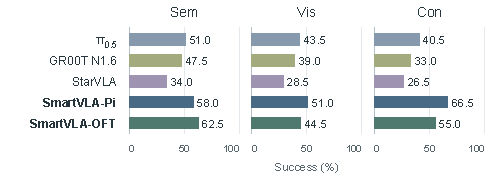
\includegraphics[width=\linewidth]{figures/fig4_piper_results.pdf}\par\nointerlineskip
\caption{Real-robot instruction following on Piper (\%).}
\label{fig:piper-results}
\end{wrapfigure}
%

% Retain the style's line-breaking settings in the wrapped paragraph.
\begingroup
\leavevmode
Beyond simulation, we evaluate fine-grained semantic following, multimodal instruction
understanding, and mid-execution corrective control on a bimanual Piper platform.
Each category contains
10 tasks, with 20 trials per task, for a total of 600 trials per model. The
tasks build on basic operations such as grasping, placing, moving, and
holding, varying language requirements, visual targets, or commands during
execution to test whether policies adjust their behavior to the current
instruction. Models use matched tasks, initial conditions, and interaction
budgets, with results reported separately for the three capabilities in
Figure~\ref{fig:piper-results}. Representative execution
trajectories are provided in Appendix~\ref{appendix:real-robot-piper}.
\par
\endgroup

In the bimanual Piper evaluation, SmartVLA-Pi and SmartVLA-OFT achieve
average success rates of 58.50\% and 54.00\%, respectively, exceeding
the strongest baseline, $\pi_{0.5}$ (45.00\%), by 13.50 and 9.00 percentage
points. On Semantic, Visual Prompt, and Control, the best result across
the two variants exceeds $\pi_{0.5}$ by 11.50, 7.50, and 26.00 percentage
points, respectively. These results show that SmartVLA also improves
fine-grained semantic following, multimodal instruction understanding,
and mid-execution corrective control in real-robot manipulation, rather
than only improving performance on simulation benchmarks.

